\documentclass[solutions]{exam}
\usepackage{graphics,color,graphicx}
\usepackage{amsmath}
\usepackage{etoolbox} %ref: https://tex.stackexchange.com/questions/161073/always-using-displaystyle-only-for-lim
\usepackage{capt-of}
\usepackage{color}
\usepackage[colorlinks=true,linkcolor=blue,urlcolor=red]{hyperref}

\apptocmd{\lim}{\limits}{}{}

\begin{document}

\begin{questions}
    \printanswers
    \CorrectChoiceEmphasis{\color{red}\bfseries}
    
        
    \question The graph of $f$ is shown in the figure above. The value of $\lim_{x\rightarrow0} f\left(1-x^2\right)$ is \\
    \begin{center}
        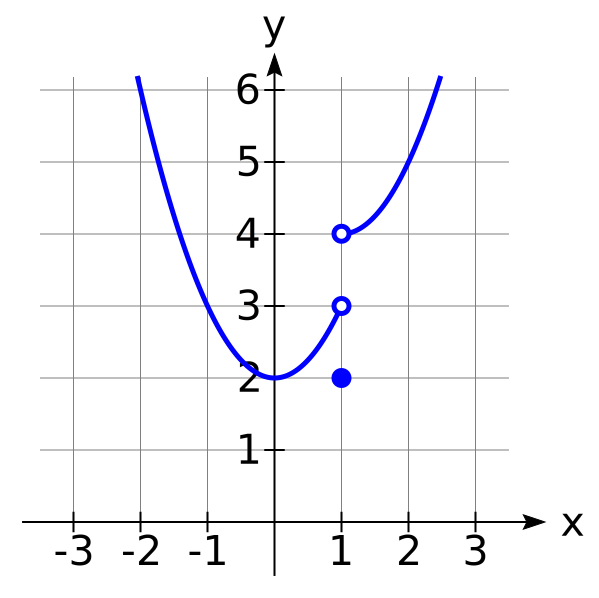
\includegraphics[width=5cm]{Q2.png}
        \captionof{figure}{Graph of $f$}
    \end{center}

    \begin{oneparchoices}
        \choice 1
        \choice 2
        \CorrectChoice 3
        \choice 4
        \choice does not exist
    \end{oneparchoices}
    \begin{solution}
        Consider the graph of $g(x)=1-x^2$. As $x\rightarrow 0, 1-x^2 \rightarrow 1$ \emph{from the left}.  Thus, we want the left-hand limit and $\lim_{x\rightarrow 0^-} f(x)=3$. \\
        Source: IPE 2016 Calculus BC \#88
        \href{https://www.youtube.com/watch?v=H5PVBDLolIs}{bpr video}
    \end{solution}
\end{questions}

\end{document}